\documentclass{Configuration_Files/PoliMi3i_thesis}

%------------------------------------------------------------------------------
%	REQUIRED PACKAGES AND  CONFIGURATIONS
%------------------------------------------------------------------------------

% CONFIGURATIONS
\usepackage{parskip} % For paragraph layout
\usepackage{setspace} % For using single or double spacing
\usepackage{emptypage} % To insert empty pages
\usepackage{multicol} % To write in multiple columns (executive summary)
\setlength\columnsep{15pt} % Column separation in executive summary
\setlength\parindent{0pt} % Indentation
\raggedbottom  

% PACKAGES FOR TITLES
\usepackage{titlesec}
% \titlespacing{\section}{left spacing}{before spacing}{after spacing}
\titlespacing{\section}{0pt}{3.3ex}{2ex}
\titlespacing{\subsection}{0pt}{3.3ex}{1.65ex}
\titlespacing{\subsubsection}{0pt}{3.3ex}{1ex}
\usepackage{color}

% PACKAGES FOR LANGUAGE AND FONT
\usepackage[english]{babel} % The document is in English  
\usepackage[utf8]{inputenc} % UTF8 encoding
\usepackage[T1]{fontenc} % Font encoding
\usepackage[11pt]{moresize} % Big fonts

% PACKAGES FOR IMAGES
\usepackage{graphicx}
\usepackage{transparent} % Enables transparent images
\usepackage{eso-pic} % For the background picture on the title page
\usepackage{subfig} % Numbered and caption subfigures using \subfloat.
\usepackage{tikz} % A package for high-quality hand-made figures.
\usetikzlibrary{}
\graphicspath{{./Images/}} % Directory of the images
\usepackage{caption} % Coloured captions
\usepackage{xcolor} % Coloured captions
\usepackage{amsthm,thmtools,xcolor} % Coloured "Theorem"
\usepackage{float}

% STANDARD MATH PACKAGES
\usepackage{amsmath}
\usepackage{amsthm}
\usepackage{amssymb}
\usepackage{amsfonts}
\usepackage{bm}
\usepackage[overload]{empheq} % For braced-style systems of equations.
\usepackage{fix-cm} % To override original LaTeX restrictions on sizes

% PACKAGES FOR TABLES
\usepackage{tabularx}
\usepackage{longtable} % Tables that can span several pages
\usepackage{colortbl}

% PACKAGES FOR ALGORITHMS (PSEUDO-CODE)
\usepackage{algorithm}
\usepackage{algorithmic}

% PACKAGES FOR REFERENCES & BIBLIOGRAPHY
\usepackage[colorlinks=true,linkcolor=black,anchorcolor=black,citecolor=black,filecolor=black,menucolor=black,runcolor=black,urlcolor=black]{hyperref} % Adds clickable links at references
\usepackage{cleveref}
\usepackage[square, numbers, sort&compress]{natbib} % Square brackets, citing references with numbers, citations sorted by appearance in the text and compressed
\bibliographystyle{abbrvnat} % You may use a different style adapted to your field

% OTHER PACKAGES
\usepackage{pdfpages} % To include a pdf file
\usepackage{afterpage}
\usepackage{lipsum} % DUMMY PACKAGE
\usepackage{fancyhdr} % For the headers
\fancyhf{}

% Input of configuration file. Do not change config.tex file unless you really know what you are doing. 
% Define blue color typical of polimi
\definecolor{bluepoli}{cmyk}{0.4,0.1,0,0.4}

% Custom theorem environments
\declaretheoremstyle[
  headfont=\color{bluepoli}\normalfont\bfseries,
  bodyfont=\color{black}\normalfont\itshape,
]{colored}

% Set-up caption colors
\captionsetup[figure]{labelfont={color=bluepoli}} % Set colour of the captions
\captionsetup[table]{labelfont={color=bluepoli}} % Set colour of the captions
\captionsetup[algorithm]{labelfont={color=bluepoli}} % Set colour of the captions

\theoremstyle{colored}
\newtheorem{theorem}{Theorem}[chapter]
\newtheorem{proposition}{Proposition}[chapter]

% Enhances the features of the standard "table" and "tabular" environments.
\newcommand\T{\rule{0pt}{2.6ex}}
\newcommand\B{\rule[-1.2ex]{0pt}{0pt}}

% Pseudo-code algorithm descriptions.
\newcounter{algsubstate}
\renewcommand{\thealgsubstate}{\alph{algsubstate}}
\newenvironment{algsubstates}
  {\setcounter{algsubstate}{0}%
   \renewcommand{\STATE}{%
     \stepcounter{algsubstate}%
     \Statex {\small\thealgsubstate:}\space}}
  {}

% New font size
\newcommand\numfontsize{\@setfontsize\Huge{200}{60}}

% Title format: chapter
\titleformat{\chapter}[hang]{
\fontsize{50}{20}\selectfont\bfseries\filright}{\textcolor{bluepoli} \thechapter\hsp\hspace{2mm}\textcolor{bluepoli}{|   }\hsp}{0pt}{\huge\bfseries \textcolor{bluepoli}
}

% Title format: section
\titleformat{\section}
{\color{bluepoli}\normalfont\Large\bfseries}
{\color{bluepoli}\thesection.}{1em}{}

% Title format: subsection
\titleformat{\subsection}
{\color{bluepoli}\normalfont\large\bfseries}
{\color{bluepoli}\thesubsection.}{1em}{}

% Title format: subsubsection
\titleformat{\subsubsection}
{\color{bluepoli}\normalfont\large\bfseries}
{\color{bluepoli}\thesubsubsection.}{1em}{}

% Shortening for setting no horizontal-spacing
\newcommand{\hsp}{\hspace{0pt}}

\makeatletter
% Renewcommand: cleardoublepage including the background pic
\renewcommand*\cleardoublepage{%
  \clearpage\if@twoside\ifodd\c@page\else
  \null
  \AddToShipoutPicture*{\BackgroundPic}
  \thispagestyle{empty}%
  \newpage
  \if@twocolumn\hbox{}\newpage\fi\fi\fi}
\makeatother

%For correctly numbering algorithms
\numberwithin{algorithm}{chapter}

%----------------------------------------------------------------------------
%	NEW COMMANDS DEFINED
%----------------------------------------------------------------------------

% EXAMPLES OF NEW COMMANDS
\newcommand{\bea}{\begin{eqnarray}} % Shortcut for equation arrays
\newcommand{\eea}{\end{eqnarray}}
\newcommand{\e}[1]{\times 10^{#1}}  % Powers of 10 notation

%----------------------------------------------------------------------------
%	ADD YOUR PACKAGES (be careful of package interaction)
%----------------------------------------------------------------------------
\usepackage{tcolorbox}
\usepackage{mathrsfs}

\usepackage{chngcntr} %this package turn off the chapter/section numbering 
\counterwithout{figure}{chapter} 
\counterwithout{figure}{section} 

\counterwithout{equation}{chapter}
\counterwithout{equation}{section} 

\counterwithout{algorithm}{chapter} 
\counterwithout{algorithm}{section}

\usepackage{enumitem}

%----------------------------------------------------------------------------
%	ADD YOUR DEFINITIONS AND COMMANDS (be careful of existing commands)
%----------------------------------------------------------------------------

%----------------------------------------------------------------------------
%	BEGIN OF YOUR DOCUMENT
%----------------------------------------------------------------------------
% Suppress the behavior of \cleardoublepage (this usually introduces blank pages)
\let\cleardoublepage\clearpage

\begin{document}

\fancypagestyle{plain}{%
\fancyhf{} % Clear all header and footer fields
\fancyhead[RO,RE]{\thepage} %RO=right odd, RE=right even
\renewcommand{\headrulewidth}{0pt}
\renewcommand{\footrulewidth}{0pt}}

%----------------------------------------------------------------------------
%	TITLE PAGE
%----------------------------------------------------------------------------

\pagestyle{empty} % No page numbers
\frontmatter % Use roman page numbering style (i, ii, iii, iv...) for the preamble pages

\puttitle{
    title={Hybrid Ensemble Models for Time Series Prediction}, % Title of the thesis
    name={Andrea Damiano}, % Author Name and Surname
    course={Management Engineering - Ingegneria Gestionale}, % Study Programme (in Italian)
    ID={225880},  % Student ID number (numero di matricola)
    advisor={Prof. Giovanni Bonaccorsi}, % Supervisor name
    coadvisor={}, % Co-Supervisor name, remove this line if there is none
    academicyear={2024-2025} % Academic Year
}

%----------------------------------------------------------------------------
%	PREAMBLE PAGES: ABSTRACT 
%----------------------------------------------------------------------------

\startpreamble
\setcounter{page}{1} % Set page counter to 1

% ABSTRACT 
\chapter*{Abstract} 
Here goes the Abstract in English of your thesis followed by a list of keywords.
The Abstract is a concise summary of the content of the thesis (single page of text)
and a guide to the most important contributions included in your thesis.
The Abstract is the very last thing you write.
It should be a self-contained text and should be clear to someone who hasn't (yet) read the whole manuscript.
The Abstract should contain the answers to the main scientific questions that have been addressed in your thesis.
It needs to summarize the adopted motivations and the adopted methodological approach as well as the findings of your work and their relevance and impact.
The Abstract is the part appearing in the record of your thesis inside POLITesi,
the Digital Archive of PhD and Master Theses (Laurea Magistrale) of Politecnico di Milano.
The Abstract will be followed by a list of four to six keywords.
Keywords are a tool to help indexers and search engines to find relevant documents.
To be relevant and effective, keywords must be chosen carefully.
They should represent the content of your work and be specific to your field or sub-field.
Keywords may be a single word or two to four words. 
\\
\\
\textbf{Keywords:} here, the keywords, of your thesis % Keywords


%----------------------------------------------------------------------------
%	PREAMBLE PAGES: ACKNOWLEDGMENTS 
%----------------------------------------------------------------------------

\chapter{Acknowledgments}
Recognition of individuals and organizations that contributed to your research.

%----------------------------------------------------------------------------
%	TABLE OF CONTENTS 
%----------------------------------------------------------------------------

% Prevent the "Contents" title from appearing in the ToC
\addtocontents{toc}{\protect\setcounter{tocdepth}{-1}} 
\thispagestyle{empty}
\tableofcontents % Table of contents 
\thispagestyle{empty}
\cleardoublepage
\addtocontents{toc}{\protect\setcounter{tocdepth}{2}}  % Restore the table of contents depth for the rest of the document

%-------------------------------------------------------------------------
%	THESIS MAIN TEXT
%-------------------------------------------------------------------------
\addtocontents{toc}{\vspace{2em}} % Add a gap in the Contents, for aesthetics
\mainmatter % Begin numeric (1,2,3...) page numbering

\chapter{Introduction}
Accurate forecasting of time series data has been a topic of great interest, for its many different application, such as improving the quality of decision-making processes in strategic sectors of governments and enterprises. As a result, over time many different models have been developed to achieve this goal. Statistical and Machine Learning (ML) methods have stood out in the area of time series forecasting in the course of the years. Traditional statistical linear methods, such as the ARIMA (Auto-Regressive Integrated Moving Average) model and its variants, have proven effective for capturing linear dependencies and seasonality in data. Such methods assume a linear correlation structure of time series patterns; therefore, these models may present reduced accuracy in forecasting real-world time series since these can present linear and nonlinear temporal patterns \cite{SANTOSJUNIOR2023119614}, \cite{kontopoulou2023review}. On the contrary, machine learning methods offer the flexibility to capture complex nonlinear patterns without relying on strict assumptions about the data's correlation structure, however, this models may not learn nonlinear and linear patterns equally due to misspecification of the parameters, which can lead to underfitting or overfitting. For this reason, many approaches in the literature have proposed hybrid models that combine the strengths of both statistical and machine learning methods to capture linear and nonlinear relationships in time series data \cite{zhang2003hybrid}, \cite{abraham2017hybrid}. One particularly promising approach discussed in the literature is \textbf{residual ensembling}, which involves modeling the linear and nonlinear patterns sequentially. The approach can be summarized in this way:
\begin{itemize}
    \item a classical linear model such as ARIMA is first applied to the time series to capture linear trends and seasonality
    \item the model’s predictions, denoted as $\hat{y}$ are then subtracted from the actual values $y$ to obtain the residuals, which should only contains the nonlinear patters of the data
    \item these residuals are then used as input to a machine learning model, which is designed to capture the remaining complex, nonlinear relationships
    \item the predictions of the linear model and of the ML model are then combined to get a single prediction.
\end{itemize}
The objective of the thesis is to propose an ensemble of models that combines the strengths of classical statistical models to capture linear dependencies with machine learning models and deep learning models to capture nonlinear dependencies. This methodology is visually represented in Figure \ref{fig: Residual learning}, taken from \cite{SANTOSJUNIOR2023119614}:
\begin{figure}[H]
    \centering
    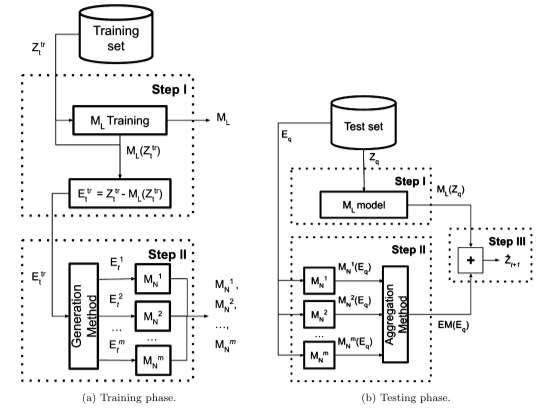
\includegraphics[width=0.50\textwidth]{Machine_learning_thesis/Images/residual learning.png}
    \caption{Residual learnign process.} 
    \label{fig: Residual learning}
\end{figure} 
Recent literature indicates that on tabular data classical machine learning approaches often outperforms deep learning methods, in particular tree ensembles, such as XGBoost, can outperforms state-of-the-art DNN models by efficiently feature-engineering the input and output structures \cite{elsayed2021do}, \cite{grinsztajn2022why}, \cite{shwartz2022tabular}. Consequently, this thesis aims to model nonlinear relationship combining tree ensemble models with deep learning models to obtain a more accurate result, as demonstrated by the following study \cite {shwartz2022tabular}. Finally, in order to combine the prediction of each base model, multiple ensemble techniques have been proposed, but the one that seems more promising and that will be used in this thesis, in order to achieve a state-of-the-art ensemble model, is named \textbf{Arbitrated Dynamic Ensemble}, proposed in following article \cite{castro2023arbitrated}, which enables to dynamically adjust the weighting of each model’s contribution based on recent patterns in the data, making the ensemble more responsive to changing trends. It consists in a meta-learner approach, designed to predict how accurate the base models will predict based on the most recent data points, which then allows to predict which model is more likely to predict well in that context, adjusting the weights as a consequence. The structure can be sumarize by the image provided by the author of the paper: 
\begin{figure}[H]
    \centering
    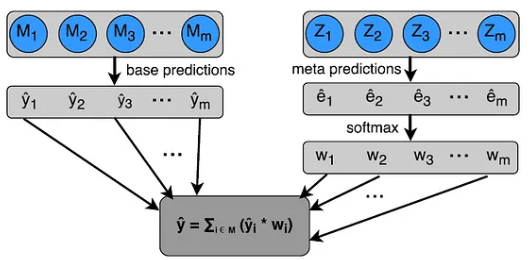
\includegraphics[width=0.50\textwidth]{Machine_learning_thesis/Images/Arbitrated Dynamic Ensemble.png}
    \caption{Arbitrated Dynamic Ensemble process.} 
    \label{fig: Arbitrated Dynamic Ensemble}
\end{figure} 
The final prediction will then be obtained as a weighted average of the weights dynamically computed: 
\[
\hat{y} = \sum_{i \in 1} \hat{y_i} w_i
\]



\chapter{Literature Review}

\section{Evolution of Time Series Forecasting}
Nowadays \textbf{Time series forecasting} has become one, if not the most, crucial tool used in decision-making and strategic planning processes across a wide range of industries such as finance, economics, environmental science, and healthcare \cite{article}. The extensive use of time series analysis in many different industries can be attributed to its ability in examining past data, detecting hidden pattern, trends and seasonality and providing insightful forecasts, which is particularly important for the businesses in order to react and prepare for upcoming events. The methodologies used has changed considerably over the years thanks to the technological innovation, in  particular, the key drivers that have spurred the progress in time series analysis have been the increase of data availability and data volume, which have been pushed by the the rise of social media, Internet of Things (IoT), and multimedia, along with the growth of cloud computing, a powerful technology that enables to perform massive-scale and complex computing eliminating the need to purchase and maintain expensive computing hardware, dedicated space, and software\cite{HASHEM201598}.
The history of time series analysis goes back to the late 19th century, with the foundational work of Francis Galton and Karl Pearson on correlation, which then posed the basis for \textbf{George Udny Yule}, a British statistician, to further advance this concepts, developing the idea of regression between two variables X and Y, without relying on the assumption that the two variables were jointly normally distributed \cite{l_kristensen_foundations_2021} and its first known application was in his 1927 with the analysis of sunspots \cite{SILVERMAN198899}, in this paper Yule developed what is now known as an autoregressive time series analysis in order to estiamate the number of sunsposts for a given year as a function of the sunspots of the two preceding years and a presumed random disturbance. This fist model was a building block for the \textbf{ARIMA} (Autoregressive Integrated Moving Average) model, later developed in the 1970s by two mathematicians, George Box and Gwilym Jenkins, in a publication called "Time Series Analysis: Forecasting and Control", with the objective of capturing the underlying patterns in time series data leveraging the three components that compose the model: autoregression, integrated, moving average. \cite{article_2}. The ARIMA model has gained a lot of popularity in the past and was one of the most commonly used approach to time series modeling as they take both long-term trends and sudden shocks into account, and many different variations where developed, to deal with the limitations of the original one, namely the ARIMAX, SARIMA, SARIMAX, VARIMA and VARIMAX models. In modern times, although ARIMA models are still being used, they are considered "classical" approaches and with the technological and statistical advancement new techniques and algorithms have been developed, capable of handling more complexed, high-dimensional, non linear time series data, leveraging machine learning and deep leaning models.


\subsection{Classical Models}  % (ARIMA, SARIMA, GARCH)}  
\subsubsection{ARIMA models}
An \textbf{ARIMA} (Autoregressive Integrated Moving Average) model, it's a more sophisticated extension of the simpler \textbf{ARMA} (Auto Regressive Moving Average) model, which combines two concepts: AR (Auto Regressive) and MA (Moving Average). 

\textbf{AR model}

Autoregressive models are regression models applied on lag series generated using the original time series. In mulitivariate linear regression, the output, the dependendent variable, is expressed as linear combination of multiple independent variables: \( y = \beta_0 + \beta_1 x_1 + \beta_2 x_2 + \cdots + \beta_n x_n + \epsilon \).
Similarly in autoregressive models with p lags or an \textbf{AR(p)} models the output (the future data point) can be expressed as a linear combination of the past p data points, where p represent the lag window: 
\begin{equation}
 y_t = \phi_1 y_{t-1} + \phi_2 y_{t-2} + \cdots + \phi_p y_{t-p} + \epsilon_t 
\end{equation}
Autoregressive models, in order to be applied, require time series to be \textbf{stationary}, which means that the statistical properties of the series, such as its mean, variance, and auto-covariance, remain constant over time. Otherwise non-stationary data can lead to unreliable model outputs and inaccurate predictions. Practically this imposes certain restrictions on the values of the autoregressive coefficients, which implies that the roots of the characteristic equation:
\begin{equation}
 1 - \phi_1 z - \phi_2 z^2 - \ldots - \phi_p z^p = 0
\end{equation}
must lie outside the unit circle, (\(|z_i| > 1 \quad\)for all roots \(z_i)\)) \cite[Section 3.2]{box1970time}.

\begin{figure}[H]
    \centering
    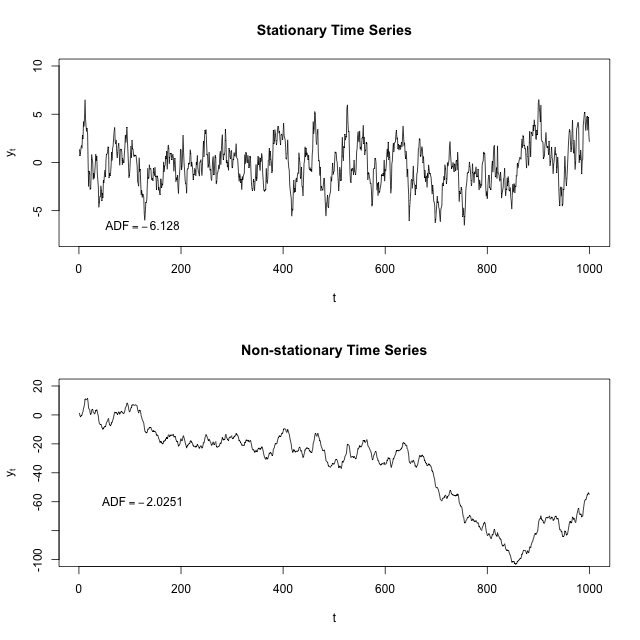
\includegraphics[width=0.50\textwidth]{Machine_learning_thesis/Images/Stationarycomparison.png}
    \caption{Example of a stationary and non-stationary process.} 
    \label{fig:Stationarycomparison}
\end{figure}

\textbf{MA model}

A moving average model uses past forecast errors in a regression-like model to predict an output(future data point), in particular, in a moving average model of order q, \textbf{MA(q)}, the ‘q’ parameter represents the number of lagged error terms to be considered in the model equation:
\begin{equation}
y_t = \mu + \varepsilon_t + \theta_1 \varepsilon_{t-1} + \theta_2 \varepsilon_{t-2} + \cdots + \theta_q \varepsilon_{t-q}
\label{MA equation}
\end{equation}
Contrary to AR(p) models, MA(q) models are stationary for any values of the coefficients \cite{chatfield2009}, indeed, if we consider the equation of a MA(q) model \eqref{MA equation}, \(y_t\) is essentially a linear combination of present and past values of \(\varepsilon_{t}\), which are assumed to be independent and identically distributed random variables with mean of zero and constant variance \( \sigma^2\), whose terms are uncorrelated. Nevertheless some constraints on the parameters of the models should be applied anyway to ensure that the model is \textbf{invertible}, which means that it can be algebraically equivalent to a converging infinite order AR model, AR(\(\infty\)), this ensure that it exists a unique MA process for a given autocorrelation function \cite{chatfield2009}. Practically this is achieved if the roots of the characteristic equation: 
\begin{equation}
 1 - \phi_1 z - \phi_2 z^2 - \ldots - \phi_p z^p = 0
\end{equation}
all lies outside the unit circle,(\(|z_i| > 1 \quad\)for all roots \(z_i)\)) \cite[pag. 50] {box1970time}.

\textbf{ARMA model}

An \textbf{ARMA(p,q)} model simply merges the two previously described models, therefore it can be expressed as: 
\begin{equation}
y_t = \mu + \phi_1 y_{t-1} + \theta_1 \epsilon_{t-1} + \epsilon_t
\end{equation}
where p and q are respectivelly the orders of the AR and MA models.

\textbf{ARIMA model}

In practise, the majority of real world time series are not stationary, and thus they must often be transformed in order to make them stationary. An \textbf{ARIMA(p, q, d)} model it's a generalizations of the autoregressive moving average (ARMA) model to non-stationary series and periodic variation with the addition of an integration component, denoted with \textbf{I(d)}, which helps  remove trends and stabilize the series in the mean sense (but it does not affect the non-stationarity of the variance or autocovariance) \cite{chatfield2009}. This can be done by differencing, which involves subtracting the preceding observation from the current one, mathematically:
\begin{equation}
 y'_t = y_t - y_{t-1}
\end{equation}
This operation is known as "first differencing",  \(\Delta\), and it is often sufficient to eliminate linear trends and achieve stationarity. If the series still shows trends or non-stationary behavior after the first pass through this process, applying "second differencing", \(\Delta^2\), may help. 
\begin{equation}
 y_t'' = (y_t - y_{t-1}) - (y_{t-1} - y_{t-2}) = y_t - 2y_{t-1} + y_{t-2}
\end{equation}
The total number of differencing is determined by the parameter d, which typically assumes the values 0, 1, 2 as higher differencing can remove too much information from the data, over-complicating the model. The generalized  ARIMA (Autoregressive Integrated Moving Average) model can be expressed mathematically as \cite{Hung2023}: 
\begin{equation}
y_t = c + \phi_1 y_{t-1} + \cdots + \phi_p y_{t-p} + \theta_1 \epsilon_{t-1} + \cdots + \theta_q \epsilon_{t-q} + \epsilon_t
\label{ARIMA equation}
\end{equation}
which can be rewritten using backshift notation as:
\begin{equation}
\Phi(B^d)(y_t - \mu) = \Theta(B)\epsilon_t
\end{equation}
where: 
\begin{itemize}

    \item \( B \) is the backshift operator such that \( B^k y_t = y_{t-k} \).
    \item \( \Phi(B^d) \) is the autoregressive polynomial of order \( p \) given by: \(\Phi(B^d) = 1 - \phi_1 B - \phi_2 B^2 - \ldots - \phi_p B^p\)
    \item \( \Theta(B) \) is the moving average polynomial of order \( q \) given by: \(\Theta(B) = 1 + \theta_1 B + \theta_2 B^2 + \ldots + \theta_q B^q\)
\end{itemize}

This model was introduce for the fist time in 1970, when the statisticians George Box and Gwilym Jenkins proposed what has become known as the Box-Jenkins method \cite{box1970time}, an approach that outlines a systematic way to identify and fit an ARIMA model to specific time series data.
\begin{figure}[H] 
    \centering
    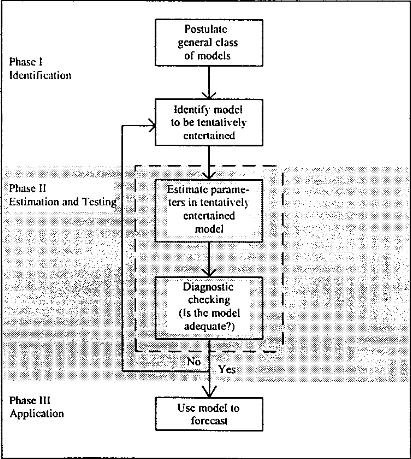
\includegraphics[width=0.4\textwidth]{Machine_learning_thesis/Images/Box_Jenkins_methodology.png}
    \caption{Schematic representation of the Box-Jenkins methodology.} 
    \label{fig:box_jenkins_methodology} 
\end{figure}

The original model used an iterative three-stage modeling approach:
\begin{enumerate}
    \item \textbf{Model Identification and Selection}: ensure the variables are stationary and identify the dependent variable's seasonality (if necessary, apply seasonal differencing). Use the plots of autocorrelation (ACF) and partial autocorrelation (PACF) functions of the dependent time series to determine which autoregressive or moving average components to use in the model.
    \item \textbf{Parameter Estimation}: utilize computation algorithms to derive the coefficients that best fit the selected ARIMA model. The most common methods for estimation are maximum likelihood estimation or non-linear least-squares estimation.
    \item \textbf{Statistical Model Checking}: test whether the estimated model conforms to the specifications of a stationary univariate process:  the residuals should be independent of each other and their mean and variance constant over time. Helpful techniques for identifying model misspecification include:
    \begin{itemize}
            \item Plotting the mean and variance of residuals over time.
            \item Performing a Ljung–Box test.
            \item Plotting the autocorrelation and partial autocorrelation of the residuals.
    \end{itemize}
    \item \textbf{Model Refinement}: if the estimation is inadequate, return to step one and attempt to build a better model.
\end{enumerate}

In empirical studies however it appears that the accuracy of such models is generally worse than much simpler time series methods. The major problem lies in the way of making the series stationary in its mean that has been proposed by Box and Jenkins. If alternative approaches are utilized to remove and extrapolate the trend in the data, ARMA models outperform the models selected through Box–Jenkins methodology \cite{Smith1997}. 

\textbf{SARIMA model}

ARIMA models do not support seasonal data, which are time series characterised by periodic fluctuations that repeats over a certain period (e.g. monthly, quarterly, yearly).
\begin{figure}[H] 
    \centering
    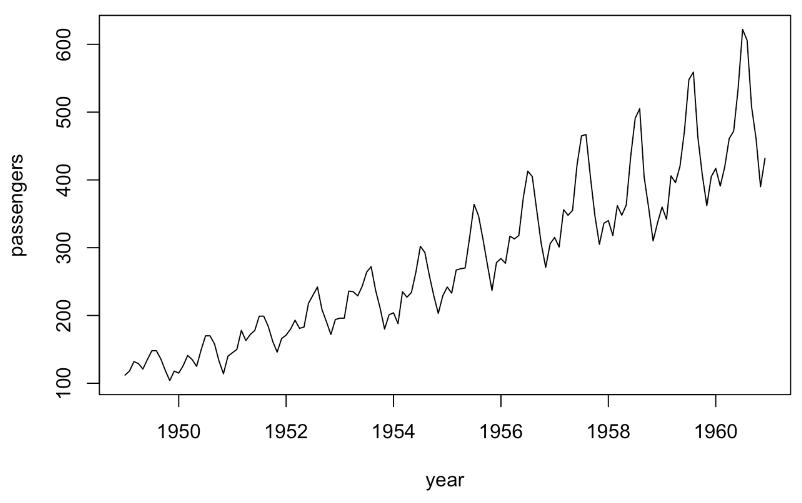
\includegraphics[width=0.4\textwidth]{Machine_learning_thesis/Images/Monthly Air Passengers(1949 - 1960).png}
    \caption{Example of a time series with seasonality (Monthly Air Passengers(1949 - 1960) Time Series).} 
    \label{fig:time_series_seasonality} 
\end{figure}
Seasonal Auto-Regressive Integrated Moving Average models, \textbf{SARIMA(p, d, q)(P, D, Q)m}, are an extension of the ARIMA (Autoregressive Integrated Moving Average) model that incorporates seasonality, by including additional seasonal terms in the ARIMA model, which are denoted by (P, D, Q)m, which represent:
\begin{itemize}
    \item P: seasonal autoregressive order
    \item D: seasonal difference order
    \item I: seasonal moving average order
    \item m: number of timesteps for a seasonal period
\end{itemize}

The general SARIMA model can be represented mathematically as follows \cite{Lee2023}:
\begin{equation}
\phi_p(B)\Phi_P(B^s)W_t = \theta_q(B)\Theta_Q(B^s)\omega_t 
\end{equation} 
where: 
\begin{itemize}
    \item \( B \): is the backshift operator, defined as \( B^k Y_t = Y_{t-k} \) 
    \item \(\phi_p(B)\): is the non-seasonal autoregressive (AR) polynomial of order p given by: \(\phi_p(B) = 1 - \phi_1 B - \phi_2 B^2 - \cdots - \phi_p B^p\)
    \item \(\Phi_P(B^s)\): is the seasonal autoregressive (SAR) component of order P given by: \(\Phi_P(B_s) = 1 - \Phi_1 B_s - \Phi_2 B_{2s} - \cdots - \Phi_P B_{Ps}\) 
    \item \(W_t\): represents the observed time series at time t. 
    \item \(\theta_q(B)\): is the \textbf{non-seasonal moving average (MA)} component of order q, give by : \(\theta_q(B) = 1 + \theta_1 B + \theta_2 B^2 + \ldots + \theta_q B^q\)
    \item \(\Theta_Q(B^s)\): is the seasonal moving average (SMA) component of order Q, given by: \(\Theta_Q(B_s) = 1 + \Theta_1 B_s + \Theta_2 B_{2s} + \ldots + \Theta_Q B_{Qs}\)
    \item \(\omega_t\): is the white noise error term at time t
\end{itemize}

\subsubsection{ARCH/GARCH}
Traditional time series models, like ARIMA models, assume costant variance over time, \textbf{homoskedasticy} \cite{MeatPrices2023}, indeed, if we look back at the formula of the ARIMA model \eqref{ARIMA equation},  \(\epsilon_t\), the white noise error term at time t is assumed to be normally distributed with mean zero and constant variance, mathematically: 
\begin{equation}
\text{Var}(\epsilon_t) = \sigma^2 \quad \text{for all } t
\end{equation}
However economic time series often shows \textbf{heteroscedasticity}, non-constant variance, that's beacuse  positive and negative news affect the variance
differently, which is known as the leverage effect. Addittionaly, economic time series often exhibit a behavior that is known as \textbf{volatility clustering}, where the volatility changes over time and its degree shows a tendency to persist. As a consequence, the dispersion of residuals changes over time, resulting in clusters of varying volatility rather than a constant spread.
\begin{figure}[H] 
    \centering
    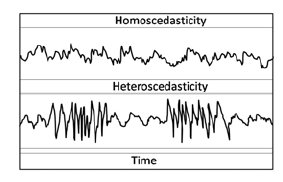
\includegraphics[width=0.5\textwidth]{Machine_learning_thesis/Images/Homoscedastic-vs-Heteroscedastic.png}
    \caption{Homoscedastic vs Heteroscedastic time series.} 
    \label{fig:Homoscedastic-vs-Heteroscedastic} 
\end{figure}
For this reason in 1982 Autoregressive Conditional Heteroscedasticity (\textbf{GARCH}) model was introduced by Robert Engle \cite{Engle1982}, to account for variance changes in financial time series by modeling the variance as a time-varying process, dependent on past errors. 

\textbf{ARCH model}

An \textbf{ARCH(p)} model is essentially an AR(p) model applied to the \textbf{conditional variance} of a time series, where p represent the order of the model, the number of past time periods used to predict the current variance at time \(t\). The conditional variance represent the variance at time \(t\), given the information of the variance untill time \(t-1\) , mathematically it is a combination of the unconditional variance and the deviation of squared error from its average value . For an ARCH(p) model it  can be represented by the following equation \cite{PalombaGARCH}: 
\begin{equation}
\displaystyle \sigma _{t}^{2}=\alpha _{0}+\alpha _{1}\epsilon _{t-1}^{2}+\cdots +\alpha _{q}\epsilon _{t-q}^{2}=\alpha _{0}+\sum _{i=1}^{q}\alpha _{i}\epsilon _{t-i}^{2}
\end{equation} 
Where:
\begin{itemize}
    \item $\sigma_{t}^{2}$ is the conditional variance at time $t$.
    \item $\epsilon _{t-i}^{2}$ are the squared residuals from previous periods.
    \item $\alpha_{0}, \dots, \alpha_{p}$ are the parameters of the model and measure the sensitivity of the conditional variance $\sigma_{t}^{2}$ to past squared residuals.
\end{itemize}

Even though conditional variance changes over time, the model can be \textbf{covariance stationary} if the variance of the process stays finite and constant over time. For an ARCH(p) model, this happenswhen the roots of the polynomial $1-A(L)$ fall outside the unit circle, this translates to the condition \cite{PalombaGARCH}: 
\begin{equation}
\sum_{i=1}^{p} \alpha_{i} < 1
\end{equation} 
where:
\begin{itemize}
    \item A(L): is the lag polynomial: \(\alpha_1 L + \alpha_2 L^2 + \cdots + \alpha_q L^q\) 
    \item L is the \textbf{lag operator}, which shifts values of the time series back by a certain number of periods 
\end{itemize}

This will ensure that shocks to the system will be dissipated instead of accumulating over time, maintaining a bounded variance and ensuring that the unconditional variance exists, assuming this value: 
\begin{equation}
\text{Var}(\epsilon_t) = \frac{\alpha _{0}}{1 - \sum_{i=1}^{q} \alpha_i}
\end{equation} 


\textbf{GARCH model}

In practice, only rather rich ARCH parameterizations are able to fit financial series adequately, however, largely parameterized models can be difficult to estimate and can bring to instability during forecasting. The Generalized Autoregressive Conditional Heteroskedasticity (GARCH) model was introduced by Tim Bollerslev in 1986 \cite{Bollerslev1986} and expands upon the ARCH model by enabling a more parsimonious approach to analyzing time-varying volatility in financial series without estimating an overly complex parameter structure. 

Unlike ARCH, which uses an autoregressive model of the past squared errors to capture volatility, the GARCH model extends this by adding the past conditional variance alongside the past squares. This is represented as a \textbf{GARCH(p, q)} model, where p and q are orders for the autoregressive and moving average terms in the variance equation, respectively. The general form for the conditional variance, \(\sigma _{t}^{2}\) , in a GARCH(p, q) model is:
\begin{equation}
\sigma_{t}^{2} = \alpha_{0} + \sum_{i=1}^{p} \alpha_{i} \epsilon_{t-i}^{2} + \sum_{j=1}^{q} \beta_{j} \sigma_{t-j}^{2}
\end{equation} 
Where: 
\begin{itemize}
    \item $\alpha_{i}$ coefficients scale past squared error terms $\epsilon_{t-i}^{2}$.
    \item $\beta_{j}$ coefficients scale past conditional variances $\sigma_{t-j}^{2}$.
\end{itemize}

The GARCH(p, q) model is covariance stationary when the roots of the polynomial \(1 - A(L) - B(L)\) fall outside the unit circle. This results in the following condition: 
\begin{equation}
\sum_{i=1}^{q} \alpha_{i} + \sum_{j=1}^{p} \beta_{j} < 1
\end{equation} 
with all parameters \(\alpha_{0}, \alpha_{i}, \beta_{i}\) being non-negative. When this condition holds, the unconditional variance of the innovation is: 
\begin{equation}
\operatorname{Var}(\epsilon_{t}) = \frac{\omega}{1 - \sum_{i=1}^{q} \alpha_{i} - \sum_{j=1}^{p} \beta_{j}}
\end{equation}


\subsection{Machine Learning models} % (Random Forest, XGBoost, LightGBM)} Subsection 2.1.2
Classical time series model, such as ARIMA and GARCH, often require specific statistical assumptions, such as stationarity of data, and if the data it's not stationary, these models usually require trasformations to stabilize variance and mean, such as differencing, to make the time series stationary. In contrast machine learning model(especially tree-base models, such as XGBooost and Ranodom Forests) are more flexible and can capture complex, non-linear patterns and dependencies in the data without requiring strict assumptions about the data's statistical properties. Study comparing ARIMA models to machine learning models show that while the first performs better in highly structured and stationary settings,the latter often delivers superior performance in dynamic environments \cite{Kontopoulou2023}.

\subsubsection{Random Forest}
\label{Sec: Random Forest}
A Random Forest model, also referred to as Random Decision Forest, is an ensemble learning model (which will be discussed in more details in the section \ref{Sec: ensemble learning}), introduced for the first time by Ho in 1995 \cite{Ho1995}, however it was Breiman who significantly advanced the methodology in 2001 \cite{Breiman2001} publishing a version that is modified and being currently used. The model developed by Leo Breiman consists of a group of un-pruned classification or regression trees made from the random selection of samples of the training data. Random features are selected in the induction process. Prediction is then made by aggregating (majority vote for classification or averaging for regression) the predictions of the ensemble. Each tree is grown as described:
\begin{itemize}
\item \textbf{Random Sampling with Replacement}: N instances will be randomly sampled from the original dataset, with replacement, meaning that some instances may appear multiple times in a single sample, while others may be omitted. This sample will then be used as the training set for growing the tree.
\item \textbf{Random Feature Selection (Feature Bagging)}: For M input variables, a subset of features m is selected (such that $m<<M$) at each split for each tree, the best split will be then selected using the m features instead of the whole M input variables. This will reduce the correlation between trees making the ensemble more robust to noise.
\item \textbf{Tree Growth Without Pruning}: each tree is grown to the largest possible extent and no pruning is used.
\end{itemize}

Random Forest generally exhibits a significant performance improvement compared to a single decision tree \cite{Sharma2015}. 

\textbf{Regression tree}

Regression trees are obtained using a \textbf{greedy}, divide and conquer algorithm that recursively partitions the given training data into smaller subsets, to minimize the prediction errors. This process, also referred to as \textbf{top-down induction} of decision trees can be described by the following procedure: 
\begin{tcolorbox}[colback=blue!5, colframe=blue!80, colframe=white, boxrule=0pt]
\begin{algorithm}[H]
    \caption{Top-down induction of decision trees}
    \label{alg:tree_construction}
    \begin{enumerate}
        \item In the initialization phase, each observation is placed in the root node of the tree. The root is included in the list \( L \) of active nodes.
        \item If the list \( L \) is empty, the procedure is stopped; otherwise, a node \( J \) belonging to the list \( L \) is selected, removed from the list, and used as the node for analysis.
        \item The optimal rule to split the observations contained in \( J \) is then determined, based on an appropriate preset criterion. The splitting rule generated in this way is then applied, and descendant nodes are constructed by subdividing the observations contained in \( J \). 
        \begin{enumerate}
            \item For each descendant node, the conditions for stopping the subdivision are verified. 
            \item If these conditions are met, node \( J \) becomes a leaf and the value assigned to it is the mean of the target values of the observations contained in \( J \). 
            \item Otherwise, the descendant nodes are added to the list \( L \). Finally, step 2 is repeated.
        \end{enumerate}
    \end{enumerate}
\end{algorithm}
\end{tcolorbox}

The procedure above is a general framework and requires some additional steps to be specified before deriving an implementable regression algorithm:
\begin{itemize}
    \item \textbf{Splitting Rules:} For each node of the tree, it is necessary to specify the criteria used to identify the optimal rule for splitting the observations and for creating the descendant nodes. There are several alternative criteria, which differ in the number of descendants, the number of attributes, and the evaluation metrics.
    \item \textbf{Stopping Criteria:} At each node of the tree, different stopping criteria are applied to establish whether the development should be continued recursively or if the node should be considered a leaf. Various criteria have been proposed for this purpose, resulting in quite different topologies of the generated trees, even if all other elements are held constant.
    \item \textbf{Pruning Criteria:} Finally, it is appropriate to apply pruning criteria to avoid excessive growth of the tree during the development phase (\textit{pre-pruning}) and to reduce the number of nodes after the tree has been generated (\textit{post-pruning}).
\end{itemize}

The trees that are usually employed in Random Forest models are \textbf{binary}, \textbf{univariate} decision trees (as described in the following papers \cite{Cutler2011}, \cite{Bernard2009}, \cite {Geurts2006}) as they offer a good balance between interpretability and predictive accuracy, and help prevent overfitting in noisy or high-dimensional datasets. These trees partition the predictor space using a sequence of binary partitions (“splits”) on individual variables.
\begin{figure}[H] 
    \centering
    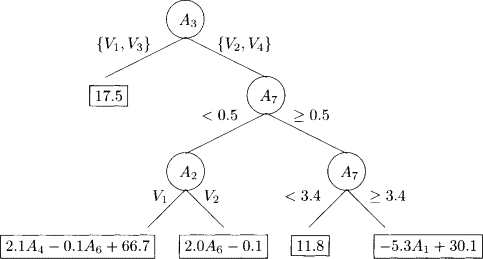
\includegraphics[width=0.5\textwidth]{Machine_learning_thesis/Images/regression tree.png}
    \caption{Example of a regression tree.} 
    \label{fig:Regression tree} 
\end{figure}
For a continuous predictor variable, a split is determined by a split-point; points for which the predictor is smaller than the split-point go to the left, the rest go to the right. 
\begin{figure}[H] 
    \centering
    \begin{tikzpicture}
        \node[anchor=center] (img) {
            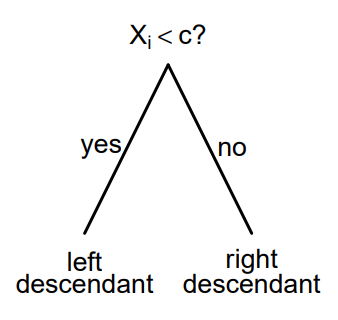
\includegraphics[width=0.3\textwidth]{Machine_learning_thesis/Images/Continuous variable split.png}
        };
        % Overlay a semi-transparent white rectangle
        \fill[white, opacity=0.2] (img.south west) rectangle (img.north east);
    \end{tikzpicture}
    \caption{Splitting on a continuous predictor variable $X_i$, using split-point $c$.} 
    \label{fig:split of a continuous variable} 
\end{figure}
The criterion used to determined the best split is the maximization of the \textbf{information gain},  $\Delta$, which is defined as: 
\begin{equation}
\Delta(q, q_1, q_2, \ldots, q_K) = I(q) - I(q_1, q_2, \ldots, q_K) = I(q) - \sum_{k=1}^{K}\frac{Q_k}{Q} I(q_k)
\end{equation}
Where: 
\begin{itemize}
    \item $I(q)$: represent the impurity index of the parent node
    \item $I(q_1, q_2, \ldots, q_K)$: represent the impurity index of the split, which is equal to the weighted sum of the impurities of each descendant node (which in the context of binary trees will be two), where each weight equals to the percentage of examples from the parent node that are placed in the corresponding descendant.  
\end{itemize}

The \textbf{heterogeneity index} (or impurity index) $I(q)$ of a node for a regression tree is a function of the variability of the target values for the examples at the node, and it has to satisfy three requirements: 
\begin{itemize}
    \item it must take its maximum value when the examples at the node are distributed homogeneously with respect to the target variable.
    \item it must take its minimum value when all the instances at the node assume the same target value.
    \item it must be a symmetric function with respect to the distribution of target values in the node.
\end{itemize}

A measure of the heterogeneity index, for regression trees, is the mean squared error: 
\begin{equation}
    I(q) = \sigma^2 = \frac{1}{N} \sum_{i=1}^{N} (y_i - \bar{y})^2
\end{equation}
Although pruning is important to prevent over-fitting for stand-alone trees, it is not used in Random Forests.

\textbf{Random Forest}
As mentioned before at the beginning of section \ref{Sec: Random Forest}, a Random Forest uses trees as base learners. Random forests are based on the concept of \textbf{bagging}, where each tree is fit to an independent \textbf{bootstrap sample} from the original data and the final prediction is obtained by averaging the results of each tree's prediction. Random Forest enhance bagging by introducing an additional level of randomness: when splitting a node, the best split is found over a randomly selected subset of $m$ predictor variables instead of all $M$ predictors, independently at each node. Two notable variations of this idea include \textbf{Forest-RI} (Random Input selection) and \textbf{Forest-RC} (Random Linear Combination selection):
\begin{itemize}
    \item Forest-RI: it randomly selects at each node, $m << M$ attributes ($m$ is fixed) as candidates for the split at the node. There is still correlation between the trees because they are based on the same observations. 
    \item Forest-RC: it represent a more radical approach, instead of using the original attributes, this method performs a perturbation which is even greater than the original dataset. It creates new attributes that are random linear combination of the existing attributes. In this way it is possible to reduce the correlation between the individual classifiers/trees. 
\end{itemize}

The process can be summirez by the following algorithm:
\begin{tcolorbox}[colback=blue!5, colframe=blue!80, boxrule=0pt]
    \begin{algorithm} [H]
        \caption{Random Forest}
        \label{alg:random_forest}
        Let $\mathscr{D} = {(x1, y1),...,(xN, yN)}$ denote the training data, with $xi = (xi,1,..., xi,p)^T$. 
        For $j = 1$ to $J$:
        \begin{enumerate}
            \item Take a bootstrap sample $\mathscr{D}_j$ of size $N$ from $\mathscr{D}$.
            \item Using the bootstrap sample $\mathscr{D}_j$ as the training data, fit a tree using binary recursive partitioning (Algorithm \ref{alg:tree_construction}).
            \begin{enumerate}
                \item Select m predictors at random from the p available predictors.
                \item Find the best binary split among all binary splits on the m predictors from step (a).
                \item Split the node into two descendant nodes using the split from step (b).
            \end{enumerate}
            \item Make a prediction at a new point $x$: 
            \[
                \hat{f}(x) = \frac{1}{J} \sum_{j=1}^{J} \hat{h}_j(x)
            \]
        \end{enumerate}
    \end{algorithm}
\end{tcolorbox}

\subsubsection{XGBoost}

\textbf{Gradient Boosting} is an ensemble machine learning technique, developed by \textbf{Jerome H. Friedman}, a statistician at Stanford University, who formalized the concept in his 2001 paper, "Greedy Function Approximation: A Gradient Boosting Machine." \cite{Friedman2001}, that consist in building multiple weak learners sequentially (typically decision trees), with each new model correcting the errors of its predecessor by placing more weights on instances with erroneous predictions, gradually minimizing a loss function. Friedman’s Gradient Boosting algorithm, often called the \textbf{Gradient Boosting Machine} (GBM), uses the gradient of a loss function, $\psi(y, f)$, to guide the correction process, iteratively estimating new models in order to optimize the predictions and minimize the loss. At each step the algorithm compute the \textbf{negative gradient} of the loss function with respect to the current model $f_{t-1}(x)$ to obtain the residual errors. This negative gradient, $g_t(x_i)$, represent the the direction in which the model should adjust to reduce loss:
\[
    g_t(x_i) = -\left.\frac{\partial \psi(y_i, f(x_i))}{\partial f(x_i)}\right|_{f(x_i) = f_{t-1}(x_i)}
\]
The objectibve of the algorithm developed by Friedmann is to add a new model, $h_t(x)$, at each step $t$, that minimizes the residual errors of the current ensemble model $f_{t-1}(x)$ and the negative gradient,  $g_t(x_i)$, of the loss function evaluated at the current model serves as a proxy for these residuals. The algorithm can be summarized by the following:
\begin{tcolorbox}[colback=blue!5, colframe=blue!80, boxrule=0pt]
    \begin{algorithm} [H]
        \caption{Friedman’s Gradient Boost algorithm}
        \label{alg:gradient boosting}
        \textbf{Inputs:}
        \begin{itemize}
            \item input data $(x, y)_{i=1}^{N}$
            \item number of iterations $M$
            \item choice of the loss-function $\psi(y, f)$
            \item choice of the base-learner model $m(x, \theta)$
        \end{itemize}

        \textbf{Algorithm:}
        \begin{enumerate}
            \item initialize $\hat{f}_0$ with a constant, often  $c=mean(y)$ for regression tasks
            
        For $t=1$ to $M$ steps
            
            \item compute the negative gradient $g_t(x_i)$ for each istance $i$
            \item fit a new base-learner function $m(x, \theta_t)$ on the negative gradients $g_t(x_i)$ to approximate them.
            \item find the best gradient descent step-size $\rho_t$:
            \[
            \rho_t = \arg \min_{\rho} \sum_{i=1}^{N} \psi[( y_i, \hat{f}_{t-1}(x_i) +\rho m(x_i, \theta_t) ]
            \]
            \item update of the function estimate:
            \[
            \hat{f}_t \leftarrow \hat{f}_{t-1} + \rho_t m(x, \theta_t)
            \]
        \end{enumerate}
    \end{algorithm}
\end{tcolorbox}



\textbf{XGBoost} 

The Extreme Gradient Boosting (XGBoost) model is a popular implementation of the Gradient Boosting general framework previously described. It was developed by \textbf{Tianqi Chen}, who introduced the model in a seminal paper titled "XGBoost: A Scalable Tree Boosting System" \cite{chen2016xgboost}. It builds on the traditional Gradient Boosting by introducing some additional features:
\begin{enumerate}
    \item \textbf{Regularization in the objective function}: the objective function include some additional regularization terms to prevent overfitting: 
    \[
    \psi(y, f) = \sum_{i} l(y_i, \hat{y}_i) + \sum_{k} \Omega(m_k)
    \]
    Where: 
    \begin{itemize}
        \addtolength{\leftskip}{2em}
        \item $l(y_i, \hat{y}_i)$ is the original loss function also present in standard Gradient Boosting.
        \item $\sum_{k} \Omega(m_k)$ is a regularization function applied to each tree $h_k$ in the model.
    \end{itemize}

    $\Omega$ is a regularization parameter that penalizes the complexity of each tree booster, taking the form:
    \[
    \Omega(m_k) = \gamma T + \frac{1}{2} \lambda \|w\|^2
    \]
    Where: 
    \begin{itemize}
        \addtolength{\leftskip}{2em}
        \item $T$ is the number of leaf nodes
        \item $\|w\|^2$ is the squared sum of the leaf prediction values
        \item $\gamma$ penalizes the number of leaf nodes
        \item $\lambda$ is the L-2 regularization parameter for leaf predicted values
    \end{itemize}

    \item \textbf{Second order Gradietn aproximation}: XGBoost uses \textbf{Newton’s method}, rather than gradient descent, to guide each round of boosting. Suppose that we have already fitted $t-1$ models, if we add a new tree booster $m_t$ to our model, the objective function would be: 
    \[
    L^{(t)} = \sum_{i=1}^n l(y_i, \hat{y}_i^{(t-1)} + m_t(\mathbf{x}_i)) + \Omega(H_t)
    \]
    So in order to choose a model $h_t$ that reduces the loss we want: 
    \[
    l(y_i, \hat{y}_i^{(t-1)} + m_t(\mathbf{x}_i)) \le l(y_i, \hat{y}_i^{(t-1)})
    \]
    which can be approximied by the second order Taylor series around the point $\hat{y}_i^{(t-1)}$:
    \[
    l(y_i, \hat{y}_i^{(t-1)} + m_t(\mathbf{x}_i)) \approx l(y_i, \hat{y}_i^{(t-1)}) + g_i m_t(\mathbf{x}_i) + \frac{1}{2} h_i m_t(\mathbf{x}_i)^2
    \]
    Where: 
    \begin{itemize}
        \addtolength{\leftskip}{2em}
        \item $g_i = \frac{\partial}{\partial \hat{y}_i^{(t-1)}} l(y_i, \hat{y}_i^{(t-1)})$ is the first order partial derivative, the \textbf{gradient}.
        \item $h_i = \frac{\partial}{\partial^2 \hat{y}_i^{(t-1)}} l(y_i, \hat{y}_i^{(t-1)})$ si the second order partial derivative, the  \textbf{hessian}.
    \end{itemize}

    \item \textbf{Missing Values and Sparsity-Aware Split Finding}: XGBoost introduces a modified algorithm for tree split finding which explicitly handles missing feature values. If some feature values are missing, the XGBoost split finding algorithm scores each threshold twice: once with missing value instances in the left node and once with them in the right node. The best split will then specify both the threshold value and to which node instances with missing values should be assigned. 

    \item \textbf{Preventing Further Splitting}: XGBoost offers some additional parameter for limiting tree splitting, preventing overfitting, a key one being the \texttt{minimum child weight} parameter, which specifies the minimum sum of the instance weights (the Hessians) in a child node.

    \item \textbf{Sampling}: XGBoost introduces both column and row subsampling, which can prevent overfitting and reduce training time by limiting the amount of data to be processed during boosting.

    \item \textbf{Scalability}: XGBoost is highly scalable thanks to the efficient, parallelizable, and distributable methods for growing trees. It allows infact to choose from different tree growth methods through the \texttt{tree\_method} parameter, which allows to choose between the greedy exact algorithm and the approximate algorithm, which offers various scalability-related functionality as the ability to consider only a small number of candidate split points instead of trying all possible splits. 
        
\end{enumerate} 


\subsection{Advances in Deep Learning} %(LSTM, GRU, CNN)}
Deep learning is a subset of machine learning that uses artificial neural networks to process and analyze information. 
\begin{figure}[H] 
    \centering
    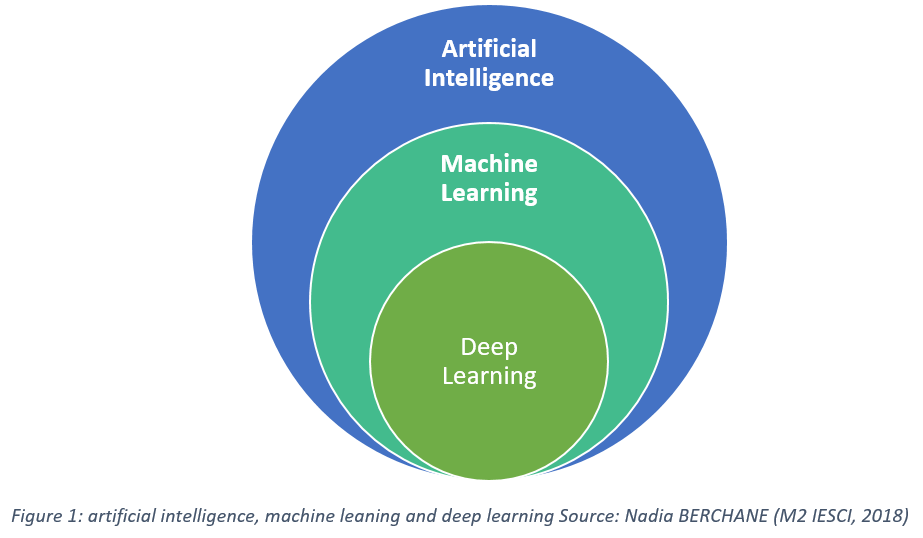
\includegraphics[width=0.6\textwidth]{Machine_learning_thesis/Images/deep learning and machine learning.png}
    \caption{Artificial intelligence, machine learning and deep learning.} 
    \label{fig:Artificial intelligence, machine learning and deep learning} 
\end{figure}

\textbf{Perceptron}

The perceptron, developed by Frank Rosenblatt in 1958 \cite{rosenblatt1958perceptron}, marked the birth of neural networks. It is the simplest form of neural network and corresponds to a single neuron, specifically deisgned for binary classification problems, that receives as input the values $(x_1, x_2, \dots, x_n)$ along the incoming connections, and returns an output value $f(x)$.
\begin{figure}[H] 
    \centering
    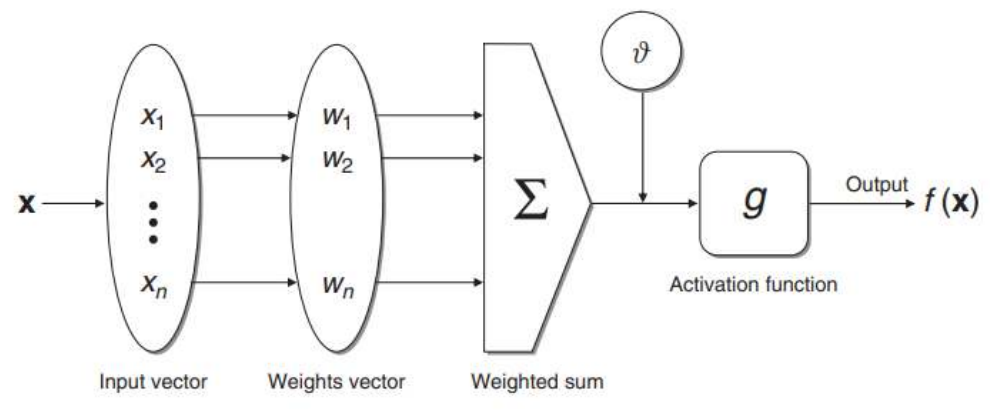
\includegraphics[width=0.4\textwidth]{Machine_learning_thesis/Images/Rosenblatt perceptron.png}
    \caption{Rosenblatt perceptron.} 
    \label{fig:Rosenblatt perceptron} 
\end{figure}
Where the input values represent the values of the explanatory attributes and the output represent the prediction of the response variable $y$. The prediction for a new observation $x$ is then derived by performing the following steps:

\begin{tcolorbox} [colback=blue!5, colframe=blue!80, boxrule=0pt]
    \begin{algorithm} [H]
        \caption{Perceptron algorithm | Part 1}
        \label{alg: Rosenblatt perceptron}
        \begin{enumerate}
            \item Each new observation $x = \{x_1, x_2, \dots, x_n\}$ is associated with a weight $w = \{w_1, w_2, \dots, w_n\}$ and a bias term $\theta$, called distortion. The perceptron first computes the \textbf{weighted linear combination} of the values of the explanatory variables for the new observation, and the distortion is subtracted from it:
            \[
            w_1 x_1 + w_2 x_2 + \dots + w_n x_n - \vartheta = \mathbf{w}' \mathbf{x} - \vartheta
            \]
            
            \item The prediction $f(x)$ is then obtained by applying an \textbf{activation function} $g$ to the linear combination of the predictors:
            \[
            f(\mathbf{x}) = g(w_1 x_1 + w_2 x_2 + \dots + w_n x_n - \vartheta) = g(\mathbf{w}' \mathbf{x} - \vartheta)
            \]
            The purpose of the activation function $g$ is to map the linear combination into the set $\mathcal{H} = \{v_1, v_2, \dots, v_h\}$ of the values assumed by the target variable, usually by means of a sigmoid profile. For binary classification problems, we have $\mathcal{H} = \{-1, 1\}$, so that one may select $g(\cdot) = \operatorname{sgn}(\cdot)$, making the prediction coincide with the sign of the weighted sum:
            \[
            f(\mathbf{x}) = \operatorname{sgn}(w_1 x_1 + w_2 x_2 + \dots + w_n x_n - \vartheta) = g(\mathbf{w}' \mathbf{x} - \vartheta)
            \]
        \end{enumerate}
    \end{algorithm}
\end{tcolorbox}    

\newpage
    
\begin{tcolorbox} [colback=blue!5, colframe=blue!80, boxrule=0pt]
    \begin{algorithm} [H]
    \setcounter{algorithm}{3}
    \caption{Perceptron algorithm | Part 2}
    \addtolength{\leftskip}{2em}
        Where $g$ is the step function: 
        \[
        g(z) = 
        \begin{cases} 
              1 & \text{if } z \geq 0 \\
             -1 & \text{if } z < 0 
        \end{cases}
        \]
        In this case, the purpose of the activation function $g$ is to establish if the point associated with the example $x_i$ is placed in the lower or upper halfspace with respect to the separating hyperplane. Hence, the Rosenblatt perceptron corresponds to a linear separation of the observations based on the target class.
        \begin{enumerate}
        \setcounter{enumi}{2}  % Start the enumeration from 3
            \item The model adjusts the weights, $\mathbf{w}$, of all the arcs and the bias, $\vartheta$, in order to minimize the error, $y_i - \hat{y}_i$, using the formulas:
            \[
            \mathbf{w_{t+1}} = \mathbf{w_t} + \eta (y_i - \hat{y}_i) \mathbf{x}_i
            \]
            \[
            \vartheta = \vartheta - \eta (y_i - \hat{y}_i)
            \]
            Where $\eta$ represents the learning rate, controlling the magnitude of the adjustments and $\hat{y}_i = f(x_i)$ is the model's prediction.
        \end{enumerate}
    \end{algorithm}
\end{tcolorbox}

\textbf{Feed-forward neural network}

A multi-level feed-forward neural network, shown in the figure below, is a more complex structure than the perceptron, which includes the following components:
\begin{itemize}
    \item \textbf{Input nodes}: receive as input the values of the explanatory attributes for each observation. Usually, the number of input nodes equals the number of explanatory variables.
    \item \textbf{Hidden nodes}: apply given transformations to the input values inside the network. Each node is connected to incoming arcs that go from other hidden nodes or from input nodes, and it is connected with outgoing arcs to output nodes or to other hidden nodes.
    \item \textbf{Output nodes}: receive connections from hidden nodes or from input nodes and return an output value that corresponds to the prediction of the response variable. In classification problems, there is usually only one output node.
\end{itemize}
\begin{figure}[H] 
    \centering
    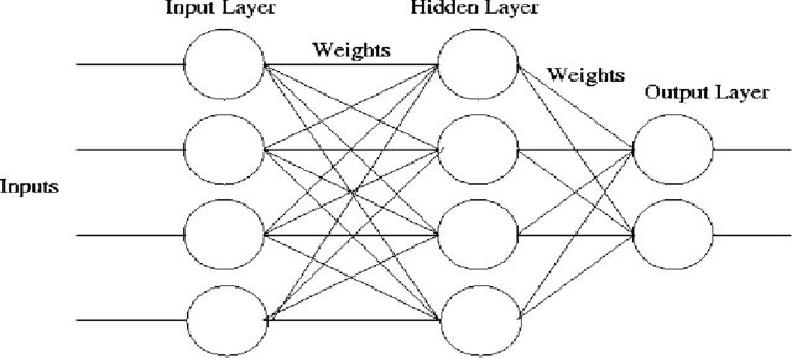
\includegraphics[width=0.6\textwidth]{Machine_learning_thesis/Images/feed-forward neural network.png}
    \caption{Feed-forward neural network.} 
    \label{fig: Feed-forward neural network} 
    \end{figure}
Each node of the network basically operates as a perceptron, in the sense that given weights are associated with the input arcs, while each node is associated with a distortion coefficient and an activation function. Each node in a multi-layer neural network extends the capabilities of the original Rosenblatt perceptron by introducing several key innovations:
\begin{itemize}
    \item use of \textbf{gradient descent} to perform the adjustments of the weights of the archs and the bias of the nodes, an idea developed in 1986, presented in the paper "Learning representations by back-propagating errors" \cite{rumelhart1986learning}. Which can be summarized by the following steps:
    
    \begin{tcolorbox} [colback=blue!5, colframe=blue!80, boxrule=0pt]
        \begin{algorithm} [H]
        \setcounter{algorithm}{4}
        \caption{Gradient descent algorithm | Part 1 }
        \label{alg: gradient descent}
        \begin{enumerate}
            \item  the inputs are forward propagated through each neuron and an output is produced (see algoritm \ref{alg: Rosenblatt perceptron} for the forward pass trough a single neuron)
            \item instead of using directly the error computed as $(y_i - \hat{y}_i)$ to update the weights of the model, a differentiable \textbf{loss function} $L(w)$, is computed, making it posible to apply the gradient descent optimization technique. A differentiable function is required because gradient-based optimization relies on the gradient, which are the partial derivatives of the loss function with respect to the model parameters. The gradient provides the direction in which the weights should be adjusted to minimize the loss function. For regression task the mean squared error (MSE) is typically used: 
            \[
            L(w) = \sum_{i=1}^{N} (y_i - \hat{y}_i)^2
            \]
        \end{enumerate}
        \end{algorithm}
    \end{tcolorbox}    

\newpage
    
\begin{tcolorbox} [colback=blue!5, colframe=blue!80, boxrule=0pt]
    \begin{algorithm} [H]
    \setcounter{algorithm}{4}
    \caption{Gradient descent algorithm| Part 2}
    \begin{enumerate}
    \setcounter{enumi}{2}
            \item the gradients of the loss function $L(w)$ with respect to the parameters of the model are computed through a process called \textbf{backpropagation}, which involves computing the gradients starting form the output layer going back untill the input layer, through the following steps:
            %\addtolength{\leftskip}{2em}
            \begin{itemize}
                \item the process begin by computing the gradients of the output layer based on the difference between the predicted output $\hat{y_i}$ and the actual target $y_i$, obtaining the error term $\delta_j^m$ ($m$ is the output layer and $j$ is the node):
                \[
                \delta_1^m = g_o'(a_1^m)(\hat{y}_d - y_d)
                \]
                Where $g_o'(\cdot)$ is the derivative of the output layer’s activation function and $a_1^m$ is the activation in the output layer.
                \item For each hidden layer k, the error term $\delta_j^k$ is computed based on the error from the subsequent layer:
                \[
                \delta_j^k = g'(a_j^k) \sum_{l=1}^{r_{k+1}} w_{jl}^{k+1} \delta_l^{k+1}
                \]
                Where $w_{jl}^{k+1}$ represent the weight between neuron $j$ in layer $k$ and neuron $l$ in layer $K+1$, and $\delta_l^{k+1}$ is the error term from the next layer.

                \item finally the gradients of the loss function with respect to the weights of the input layer are computed:
                \[
                \frac{\partial w_{ij}^k}{\partial L} = \delta_j^k \cdot o_i^{k-1}
                \]
                Where $o_i^{k-1}$ represent the input feature value
            \end{itemize}
            \item once all the gradients are computed, the weights of the model at each layer are updated using a gradient descent approach, the most common being: 
            \[
            w_{ij}^k \leftarrow w_{ij}^k - \eta \frac{\partial w_{ij}^k}{\partial L}
            \]
            Where $\eta$ is the earning rate, controlling the step size for each update.
        \end{enumerate}
        \end{algorithm}
    \end{tcolorbox}


    \item feed farward neural network employs more complex nonlinear activation functions, which ensure the model to capture complex patterns in data. Two of the most commonly used activation fuction for hidden layers are the ReLu (Rectified Linear Unit) and the Tanh (Hyperbolic Tangent) functions, whereas the Sigmoid and the Softmax funtion are typically used for the output nodes for classification problems, converting the otuputs of the nutwork into prediction probabilities:  
    \[
    g(z) = \text{ReLU}(z) = \max(0, z)
    \]
    \[
    g(z) = \tanh(z) = \frac{e^z - e^{-z}}{e^z + e^{-z}}
    \]
    \begin{figure}[H] 
    \centering
    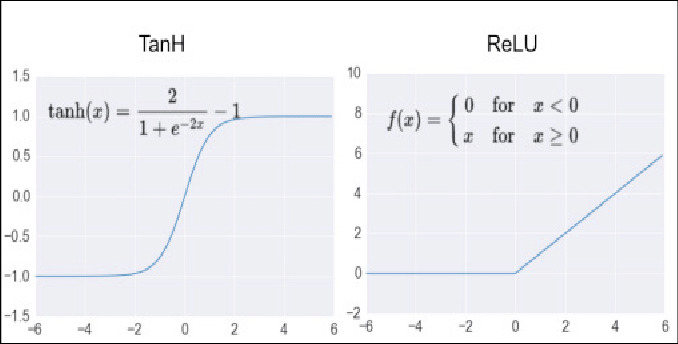
\includegraphics[width=0.6\textwidth]{Machine_learning_thesis/Images/Tanh-and-ReLU-activation-functions.png}
    \caption{Tanh and ReLU activation functions.} 
    \label{fig:Tanh and ReLU activation functions} 
    \end{figure}

    \[
    \sigma(z) = \frac{1}{1 + e^{-z}}
    \]
    \[
    g(z) = \text{softmax}(z) = \frac{e^{z}}{\sum_{j=1}^n e^{z}}
    \]
    \begin{figure}[H] 
    \centering
    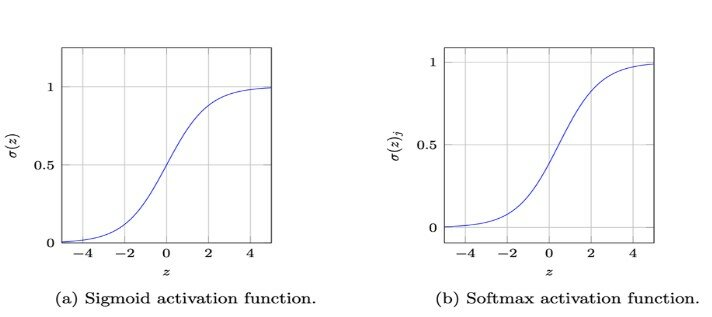
\includegraphics[width=0.6\textwidth]{Machine_learning_thesis/Images/sigmoid and softmax functions.png}
    \caption{Sigmoid and Softamx activation functions.} 
    \label{fig:Sigmoid and Softamx activation functions} 
    \end{figure}
    
\end{itemize}

\subsubsection{LSTM model}
The \textbf{Long Short-Term Memory} (LSTM) model is a type of \textbf{Recurrent Neural Network} (RNN), originally introduced by  Sepp Hochreiter and Jürgen Schmidhuber in 1997 in the paper "Long Short-term Memory" \cite{hochreiter1997long}. The model was developed in order to address the limitation of traditionals RNN models. 

\textbf{Recurrent Neural network}

It's a type of artificial neural network specifically design for processing sequential data, where each input depends on previous elements in the sequence. Unlike traditional feed-forward neural networks where all  inputs and outputs are treated indipendently, RNN models introduce an \textbf{hidden state}, that retains some information from earlier steps in the sequence, allowing the model to "remember".
\begin{figure}[H]
    \begin{minipage}{0.3168\textwidth}
        \centering
        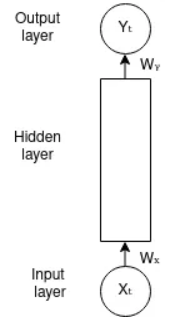
\includegraphics[width=\textwidth]{Machine_learning_thesis/Images/FeedForward Neural Network.png}
        \caption{Feed-forward neural network.}
        \label{fig:image1}
    \end{minipage}%
    \hfill
    \begin{minipage}{0.418\textwidth}
        \centering
        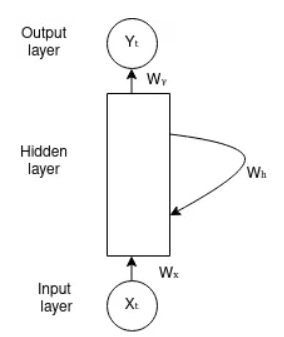
\includegraphics[width=\textwidth]{Machine_learning_thesis/Images/Recurrent Neural Network.png}
        \caption{Recurrent neural network.}
        \label{fig:image2}
    \end{minipage}
\end{figure}
At each time step $t$, the hidden state $h_t$ is computed based on the current input $x_t$ and the previous hidden state $h_{t-1}$ as illustrated by the following formula:
\[
h_t = \sigma\left(W_{xh} x_t + W_{hh} h_{t-1} + b_h\right)
\]
Where: 
\begin{itemize}
    \item $W_{xh}$ is the weight matrix governing the connections from the hidden layer to itself (recurrent connections)
    \item $W_{hh}$ is the weight matrix governing the connections from the input to the hidden layer
    \item $b_h$ is the bias vector
    \item $\sigma$ is the activation function (typically ReLu or tahn)
\end{itemize}
The output at each time step, $y_t$, is then computed  based on the hidden state output using the following formula:
\[
\hat{y}_t = f\left(V \cdot h_t + c\right)
\]
Where: 
\begin{itemize}
    \item $V$ is the weight matrix governing the connections from the hidden layer to the output layer
    \item $c$ is the bias vector
\end{itemize}
However RNN models, struggle with long-term dependencies due to issues like the \textbf{vanishing gradient} problem, which consists in gradients becoming too small during backpropagation, making it hard to retain information from earlier steps. Another common problem is the \textbf{exploding gradient} problem, where gradients become excessively large during backpropagation causing the model's parameters to update erratically leading to instbility and the model to deviate from the optimal solution and making it difficult for the network to converge to global minima.

\textbf{Long Short-Term Memory}

The LSTM model is a modified version of recurrent neural networks,that addresses key limitations in handling long-term dependencies. The core of the model is the \textbf{Cell state}, which serves as a long-term memory for the model carrying the information straight through the network, from one time step to the next.
\begin{figure}[H] 
    \centering
    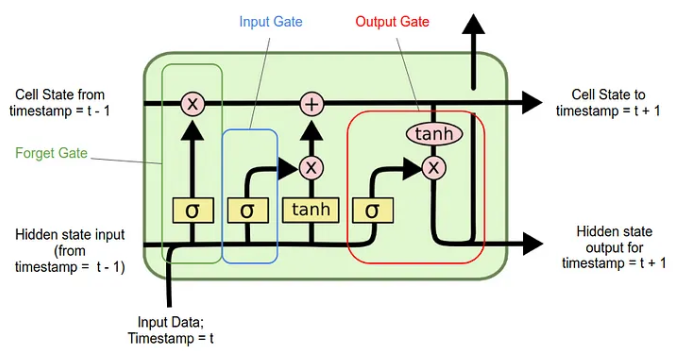
\includegraphics[width=0.6\textwidth]{Machine_learning_thesis/Images/LSTM cell.png}
    \caption{Long Short Memory cell.} 
    \label{fig:LSTM cell} 
\end{figure}
The models uses gates to manage the flow of information, within the cell state, enabling it to selectively retain, update, or discard information at each time step, as a result, not all time-steps are incorporated equally into the cell state. To perform this the model employs three gates:
\begin{itemize}
    \item \textbf{Forget gate}: looks at the current input and the previous hidden state (which carries past information, acting as a short-term memory for the model) and decides what information to forget, giving an output that goes from 0 (completely forget) to 1 (retain everything), it is computed as: 
    \[
    f_t = \sigma\left(W_f \cdot \left[h_{t-1}, x_t\right] + b_f\right)
    \]
    \item \textbf{Input gate}: determines what new information should be added to the cell state by giving an output that goes form 0 to 1, indicating how much information should be stored. Firstly it creates a new candidate set of information determined as: 
    \[
    \tilde{C}_t = \tanh\left(W_C \cdot \left[h_{t-1}, x_t\right] + b_C\right)
    \]
    and then chooses which parts of this will be added to the cell state, using the formula:
    \[
    i_t = \sigma\left(W_i \cdot \left[h_{t-1}, x_t\right] + b_i\right)
    \]
    \item \textbf{Output Gate}: controls what part of the cell state gets passed to the hidden state for the next time step, also returning an output from 0 to 1, using the formula:
    \[
    o_t = \sigma\left(W_o \cdot \left[h_{t-1}, x_t\right] + b_o\right)
    \]
\end{itemize}

This three gates are then employed to update both the hidden state and the cell state, respectivelly using the formulas:
\[
h_t = o_t \cdot \tanh(C_t)
\]
\[
C_t = f_t \cdot C_{t-1} + i_t \cdot \tilde{C}_t
\]

\subsubsection{1D CNN model for time series}
\textbf{Convolutionary neural network} are another popular class of artificial neural netowrk, introduced for the first time by Yann LeCun, during the development of the \textbf{LeNet} architecture\cite{lecun1989generalization}. The model was initially developed for image classification tasks, since it has the ability to learn spatial hierarchies in data through local receptive fields and weight sharing. 

\textbf{CNN model for images}

At the heart of CNNs is a mathematical operation called \textbf{convolution}, which is an operation that combines an input $I$ with a \textbf{kernel} $K$ (a filter) to produce feature maps that highlight specific data patterns. The  convolutional operation $S$ on a 2-D image e may be describe
as follows \cite{lecun1989generalization}:
\[
S(i, j) = (I \times K)(i, j) = \sum_m \sum_n I(m, n) K(i - m, j - n)
\]
The operation slides the kernel across the input data, generating outputs based on localized interactions, as shown in the figure below.
\begin{figure}[H] 
    \centering
    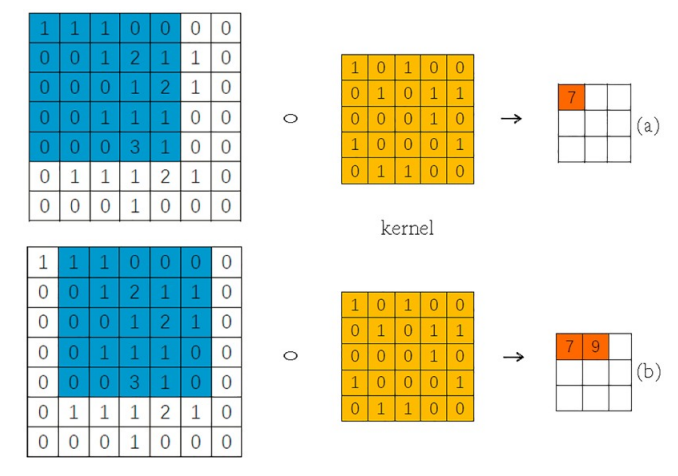
\includegraphics[width=0.6\textwidth]{Machine_learning_thesis/Images/Convolution.png}
    \caption{Example of a convolutional operation.} 
    \label{fig:convolution} 
\end{figure}
Usually after a convolution process a \textbf{pooling} operation is performed in sequence, which involve sliding a n-dimensional filter over each channel of the feature map generated by the convolutional operation, summarizing the features lying within the region covered by the filter. This is done to  reduce the number of parameters the model has to learn and the amount of computation performed in the network, making the model more robust to variations in the position of the features in the input image. The two common pooling methods are:
\begin{itemize}
    \item \textbf{Max Pooling}: which takes the maximum value from each region, capturing the most prominent feature in that region:
    \[
    y_{i,j} = \max(x_{2i:2i+2, 2j:2j+2})
    \]
    \item \textbf{Average Pooling}: which computes the average of values in each region:
    \[
    y_{i,j} = \frac{1}{4} \sum_{m=0}^{1} \sum_{n=0}^{1} x_{2i+m, 2j+n}
    \]
\end{itemize}
\begin{figure}[H] 
    \centering
    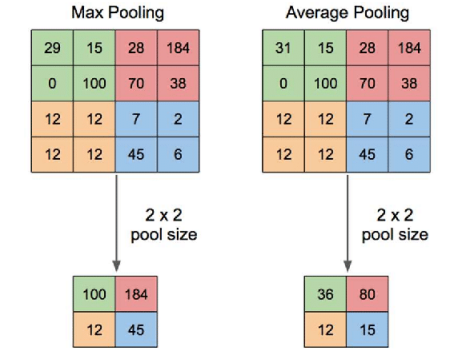
\includegraphics[width=0.6\textwidth]{Machine_learning_thesis/Images/Max pooling and Average pooling.png}
    \caption{Example of Max pooling and Average pooling operations.} 
    \label{fig:Max pooling and Average pooling} 
\end{figure}
Finally a dropout layer is often applied to avoid model overfitting. In the \textbf{dropout} operation, each hidden unit have some probability $p$ of being omitted
during the model training. In more modern approaches, different groups of hidden units have different probabilities of being omitted during training, the so-called biased dropout operation.
\begin{figure}[H] 
    \centering
    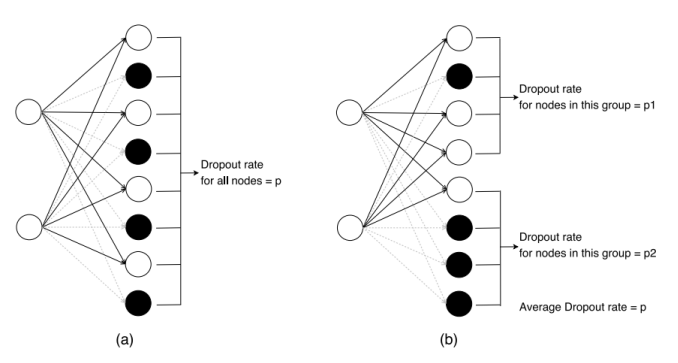
\includegraphics[width=0.6\textwidth]{Machine_learning_thesis/Images/Dropout.png}
    \caption{Regular dropout and Biased dropout layers example.} 
    \label{fig:Regular dropout and Biased dropout} 
\end{figure}


\section{Ensemble Techniques in Time Series} 
\label{Sec: ensemble learning}
\subsection{Stacking and Blending Methods} 
% Content for stacking and blending methods
\subsection{Hybrid Approaches in Time Series Forecasting}
% Content for hybrid deep learning models
\subsection{Integrating Classical and Deep Learning Models}
% Content for integrating models






\section{Gaps in Existing Research and the Need for Hybrid Solutions} 
\subsection{Addressing Non-stationarity and Volatility}
% Content for non-stationarity and volatility
\subsection{Capturing Complex Temporal Dependencies} 
% Content for temporal dependencies





\chapter{Problem definition}

\section{Defining Key Time Series Characteristics} % Section 3.1
% Content for key time series characteristics (Trend, Seasonality, Stationarity)

\section{Domain-specific Case Study} % Section 3.2
\subsection{Focus on Energy Consumption} % Subsection 3.2.1
% Content for energy consumption case study

\subsection{Focus on Financial Data} % Subsection 3.2.2
% Content for financial data case study

\section{Forecasting Challenges in the Chosen Domain} % Section 3.3
% Content for forecasting challenges

\section{Research Questions and Hypotheses} % Section 3.4
% Content for research questions and hypotheses

\chapter{Methodology}

\section{Data Preprocessing and Exploratory Data Analysis} 
\subsection{Handling Non-Stationarity} % Content for handling non-stationarity
\subsection{Feature Engineering and Temporal Feature Extraction} % Content for feature engineering


\section{Choice of Base Models}
\subsection{Statistical models}
\subsection{Tree ensembles}
\subsection{Deep leanring models}


\section{Multi-Step Forecasting}


\section{Residual Ensembling Approach}
%Steps for sequentially modeling linear and nonlinear patterns
%Details on calculating residuals and using them in machine learning models


\section{Arbitrated Dynamic Ensemble (ADE)}
\subsection{Overview} %Introduction to Arbitrated Dynamic Ensemble, a method for dynamically adjusting model weights based on recent data patterns.
\subsection{Dynamic Weighting Mechanisms} %Explanation of how ADE dynamically weights model contributions, allowing the ensemble to adapt to evolving patterns in the data.
\subsection{Role of the Meta-Learner} %Description of the meta-learner’s role in assessing model performance and optimizing ensemble weighting for improved forecast accuracy.


\section{Proposed Model Architecture} 
\subsection{Hybrid Model Composition} %Explanation of the architecture that integrates ARIMA, tree ensembles (e.g., XGBoost), and deep learning models for a comprehensive solution to model both linear and nonlinear dependencies.
\subsection{Workflow} %Step-by-step outline of the complete modeling pipeline, including training, ensembling, and applying ADE adjustments.
%End-to-End Prediction Pipeline: Summary of the end-to-end process from data preprocessing to final predictions, detailing each model’s role and the integration with ADE.


\section{Evaluation Metrics for Model Performance}
\subsection{Root Mean Square Error (RMSE)} %Selection of RMSE for its ability to penalize larger errors, particularly relevant for time series forecasting.
\subsection{Mean Absolute Error (MAE)} %Justification for using MAE to provide an overall measure of prediction accuracy based on absolute differences.




\chapter{Results and Discussion}

\section{Performance of Classical, Machine Learning, and Deep Learning Models} % Section 5.1
% Content for model performance comparison

\section{Evaluation of Hybrid Ensemble Model Performance} % Section 5.2
\subsection{Analyzing Residuals and Model Robustness} % Subsection 5.2.1
% Content for analyzing residuals

\subsection{Benchmarking with State-of-the-Art Models} % Subsection 5.2.2
% Content for benchmarking models

\section{Case Study: Energy Consumption/Financial Forecasting} % Section 5.3
\subsection{Practical Applications of the Hybrid Model} % Subsection 5.3.1
% Content for practical applications

\subsection{Comparative Analysis with Existing Forecasting Techniques} % Subsection 5.3.2
% Content for comparative analysis

\chapter{Conclusion}

\section{Summary of Findings and Contributions} % Section 6.1
% Content for summary of findings and contributions

\section{Limitations and Future Work} % Section 6.2
% Content for limitations and future work

\section{Extending the Model to Other Time Series Domains} % Section 6.3
% Content for extending the model

\section{Real-world Impact and Implications of the Hybrid Ensemble} % Section 6.4
% Content for real-world impact and implications

%-------------------------------------------------------------------------
%	BIBLIOGRAPHY
%-------------------------------------------------------------------------

\addtocontents{toc}{\vspace{2em}} % Add a gap in the Contents, for aesthetics
\bibliography{Thesis_bibliography} % The references information are stored in the file named "Thesis_bibliography.bib"

%-------------------------------------------------------------------------
%	APPENDICES
%-------------------------------------------------------------------------

\cleardoublepage
\addtocontents{toc}{\vspace{2em}} % Add a gap in the Contents, for aesthetics
\appendix

\chapter{Appendix A}
If you need to include an appendix to support the research in your thesis, you can place it at the end of the manuscript.
An appendix contains supplementary material (figures, tables, data, codes, mathematical proofs, surveys, \dots)
which supplement the main results contained in the previous chapters.

\chapter{Appendix B}
It may be necessary to include another appendix to better organize the presentation of supplementary material.


% LIST OF FIGURES
\listoffigures

% LIST OF TABLES
\listoftables

% LIST OF SYMBOLS
% Write out the List of Symbols in this page
\chapter*{List of Symbols} % You have to include a chapter for your list of symbols (
\begin{table}[H]
    \centering
    \begin{tabular}{lll}
        \textbf{Variable} & \textbf{Description} & \textbf{SI unit} \\\hline\\[-9px]
        $\bm{u}$ & solid displacement & m \\[2px]
        $\bm{u}_f$ & fluid displacement & m \\[2px]
    \end{tabular}
\end{table}

\cleardoublepage

\end{document}
